\newgeometry{
	hmargin={2.5cm,2.5cm}, % Margens esquerda (dentro) e direita (fora).
	vmargin={3cm,1cm} % Margens superior e inferior.}
}

\thispagestyle{empty}

\begin{flushleft}
	\vspace*{2cm}
	\Huge\textbf{\titulo}
\end{flushleft}

\cleardoublepage

\thispagestyle{empty}

\begin{flushleft}
	\Large \autor
	\vspace{2cm}\\
	\Huge\textbf{\titulo}
	\vspace{0.5cm}\\
	\Large\subtitulo
\end{flushleft}

	\vfill

\begin{figure}[!h]
	\centering
	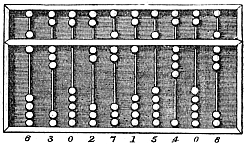
\includegraphics[scale=0.5]{./imagens/abacus}
	\caption*{\scshape Livros \& Liberdade}
	% Ideias de nomes de editora: Publicações Livres Campinas, Teoria Livre, Conhecimento Livre, Saber Livre, Livro Livre, Liber Libera/Libera Liber (Livro Livre em Latim, precisa conferir se é assim mesmo), Livr\oe, Liber \& Libertatem.
\end{figure}

\clearpage

\restoregeometry